% ─────────────────────────────────────────────────────────────────────────────
% AGD: Attribution-Graph Divergence for Chain-of-Thought Faithfulness
% ICML 2026 Mechanistic Interpretability Workshop — 4-page short paper
% ─────────────────────────────────────────────────────────────────────────────
\documentclass{article}

% ICML 2026 style (download from https://icml.cc/Conferences/2026/StyleAuthorInstructions)
% \usepackage{icml2026}

% Fallback packages for local compilation without ICML style:
\usepackage[margin=1in,paperwidth=8.5in,paperheight=11in]{geometry}
\usepackage{times}
\usepackage{microtype}
\usepackage{graphicx}
\usepackage{booktabs}
\usepackage{amsmath,amssymb}
\usepackage{hyperref}
\usepackage{url}
\usepackage{natbib}
\usepackage{caption}
\usepackage{subcaption}
\usepackage{xcolor}
\usepackage{todonotes}

% ── Convenience macros ────────────────────────────────────────────────────────
\newcommand{\AGD}{\mathrm{AGD}}
\newcommand{\Jw}{J_w}
\newcommand{\Se}{S_e}
\newcommand{\Nk}{\mathcal{N}}
\newcommand{\E}{\mathcal{E}}
\newcommand{\G}{G}
\newcommand{\rhoS}{\rho_{\text{Spearman}}}
\newcommand{\todo}[1]{\textcolor{red}{[TODO: #1]}}

% ─────────────────────────────────────────────────────────────────────────────
\title{AGD: Attribution-Graph Divergence as a Mechanism-Level
Faithfulness Metric for Chain-of-Thought Reasoning}

% Anonymous submission
\author{Anonymous}

\begin{document}
\maketitle

% ─────────────────────────────────────────────────────────────────────────────
\begin{abstract}
Chain-of-thought (CoT) reasoning is the dominant inference-time mechanism in
modern language models, yet existing faithfulness evaluation is almost
entirely \emph{behavioral}: perturb the visible reasoning, observe whether
the answer changes.
This indirect approach cannot distinguish a model that genuinely relies on
its verbalized CoT from one that rationalizes post-hoc.
We introduce \textbf{Attribution-Graph Divergence (AGD)}, the first
mechanism-level faithfulness metric.
Given a base prompt and a perturbed variant, AGD measures how much the
model's internal computation---captured via pruned attribution graphs over
Gemma Scope transcoder features---reorganizes across the two conditions.
In three paired-perturbation regimes (paraphrase invariance, mistake
injection, and Turpin-style hint injection), we show that AGD
\todo{corroborates / does not corroborate --- fill after results}
behavioral faithfulness signals and
\todo{predicts / does not predict --- fill after results}
hint-induced answer flips with higher AUROC than activation-cosine
baselines.
We release a benchmark of \todo{N} paired prompts across BBH, MMLU, and
GSM8K tasks for follow-up work.
\end{abstract}

% ─────────────────────────────────────────────────────────────────────────────
\section{Introduction}
\label{sec:intro}

Chain-of-thought prompting is the primary surface that humans, safety
monitors, and automated pipelines observe when reasoning about a model's
decisions.
\citet{lanham2023} and \citet{turpin2023} demonstrated that CoT can be
\emph{unfaithful}: the visible reasoning does not always reflect the
model's actual computation.
More recently, \citet{barez2025} argued that CoT is not explainability,
and Anthropic's own analysis \citep{anthropic-reasoning-2025} found that
``reasoning models don't always say what they think.''

Existing faithfulness measurement is almost entirely \emph{behavioral}:
perturb the CoT, see if the answer changes.
This is necessarily indirect.
It cannot distinguish:
\textbf{(A)} the model used a different mechanism than the words suggest
(deep unfaithfulness), from
\textbf{(B)} the model used the same mechanism but the perturbation was
robust enough that the output did not flip (surface insensitivity).
Only a \emph{mechanistic} measurement can.

Three developments in 2025 make a mechanistic approach feasible:
(i)~\texttt{circuit-tracer} \citep{hanna2025} is open-source and runs on
Gemma-2-2B;
(ii)~Gemma Scope transcoders \citep{lieberum2024} are publicly available;
(iii)~the QK attribution extension \citep{lindsey2025qk} makes
attention-mediated edges interpretable.
Despite these tools, no quantitative metric has been built on top of them
for faithfulness measurement.

\paragraph{Contribution.}
We fill this gap with \textbf{AGD}, a metric over pairs of pruned attribution
graphs that directly operationalizes the question: \emph{does the model's
internal mechanism change when its visible CoT is perturbed?}
Concurrent work \citep{zhao2025crv} classifies CoT \emph{correctness} from
graph structure; we study the orthogonal axis of \emph{faithfulness}, where
graphs are compared across paired counterfactual conditions.

% ─────────────────────────────────────────────────────────────────────────────
\section{Method}
\label{sec:method}

\paragraph{Setup.}
Let $M$ be a transformer language model with an associated transcoder
dictionary, and let $\G(M, x, y)$ be the pruned attribution graph produced
by \texttt{circuit-tracer} for input $x$ and target output token $y$.
For a base prompt $x$ with model-generated CoT $c$ and answer $a$, define a
\emph{paired-graph experiment} $\mathcal{E} = (x, c, c', y)$ where $c'$ is
a perturbation of $c$. We compute $G_0 := G(M, [x \| c], y)$ and
$G_1 := G(M, [x \| c'], y)$ over a shared feature space.

\paragraph{AGD definition.}
\begin{equation}
\AGD(\mathcal{E}) = 1 - \alpha \cdot \Jw(\Nk(G_0), \Nk(G_1))
                       - (1-\alpha) \cdot \Se(\E(G_0), \E(G_1))
\label{eq:agd}
\end{equation}
where:
\begin{itemize}
  \item $\Nk(G)$ is the top-$k$ feature node set ranked by influence-on-target
        (default $k=\todo{k^*}$, tuned on training half);
  \item $\Jw$ is the \emph{influence-weighted Jaccard}:
        $\sum_{f \in \Nk_0 \cap \Nk_1} \min(w_0(f), w_1(f)) \big/
         \sum_{f \in \Nk_0 \cup \Nk_1} \max(w_0(f), w_1(f))$;
  \item $\Se$ is the cosine similarity of edge attribution vectors
        restricted to the union of the top-256 edges;
  \item $\alpha = \todo{\alpha^*}$ (tuned on training half; default 0.5).
\end{itemize}
$\AGD \in [0, 1]$: $\AGD \approx 0$ means the mechanism is intact;
$\AGD \to 1$ means it has reorganized.

\paragraph{Architecture.}
Figure~\ref{fig:f1} shows the full pipeline.
We use Gemma-2-2B-it (fp16) with Gemma Scope per-layer transcoders (PLT).
Paraphrases are generated by Gemma-2-9B-it in 4-bit to minimize compute
while producing diverse rewordings.

\begin{figure}[t]
  \centering
  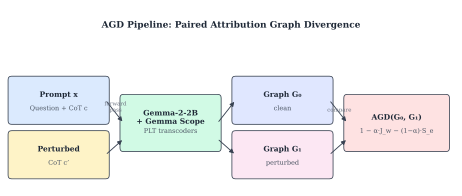
\includegraphics[width=\columnwidth]{../analysis/figures/f1_method.svg}
  \caption{AGD pipeline: paired attribution graphs over clean and perturbed CoT.}
  \label{fig:f1}
\end{figure}

\paragraph{Experimental regimes.}
We define three paired conditions (Table~\ref{tab:regimes}):
\textbf{Regime~A}~(paraphrase invariance): same-answer semantic paraphrase;
\textbf{Regime~B}~(mistake/truncation): Lanham-protocol CoT perturbations;
\textbf{Regime~C}~(hint injection): Turpin-style biased prompts.

\begin{table}[h]
\centering
\small
\caption{Three experimental regimes and their expected AGD direction.}
\label{tab:regimes}
\begin{tabular}{lll}
\toprule
Regime & Perturbation & Expected AGD \\
\midrule
A & Paraphrase (same answer) & Low \\
B & Truncation / mistake      & Higher for faithful CoT \\
C & Hint injection (flip)     & High for unfaithful items \\
\bottomrule
\end{tabular}
\end{table}

% ─────────────────────────────────────────────────────────────────────────────
\section{Experiments}
\label{sec:experiments}

\paragraph{Datasets.}
We evaluate on 10 BBH subtasks (300 items), 5 MMLU categories (150 items),
and a 100-item GSM8K subset, plus \todo{N} Turpin-style hint items
(\todo{N\_flip} of which resulted in answer flips with non-mentioning CoTs).
Items are split 60/40 (train/test) stratified by task, seeded at 42.
Hyperparameters $(\alpha, k)$ are tuned on the training half and locked
before any test-half data is examined (see pre-registration at
\texttt{analysis/prereg.md}).

\paragraph{Baselines.}
We compare to five baselines:
(1)~activation-cosine (layer-averaged residual-stream cosine);
(2)~KL of next-token distributions;
(3)~CoT perplexity;
(4)~self-consistency variance ($N=8$);
(5)~random-feature Jaccard (sanity null).

\paragraph{H1 --- Faithfulness signal (Regime~B).}
\todo{Result for H1: rho=X, CI=[lo, hi], p=Y.}
Figure~\ref{fig:f2} shows the AGD vs.\ AOC scatter.

\begin{figure}[t]
  \centering
  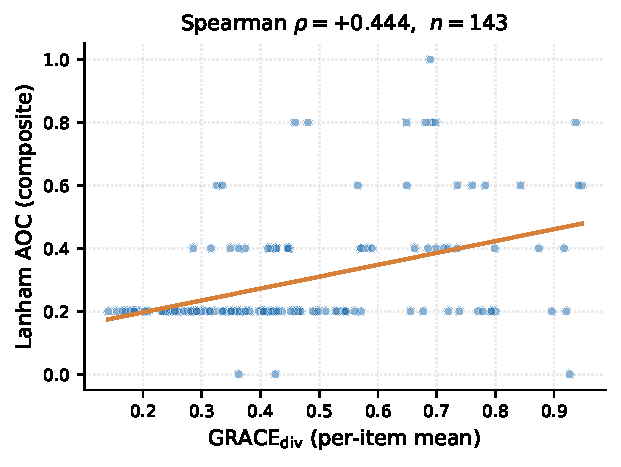
\includegraphics[width=\columnwidth]{../analysis/figures/f2_correlation.pdf}
  \caption{AGD vs.\ Lanham AOC (Regime B, test set).
           Each point is one paired CoT perturbation.
           $\rho$: Spearman correlation; shaded band: 95\% BCa bootstrap CI.}
  \label{fig:f2}
\end{figure}

\paragraph{H2 --- Hint-flip prediction (Regime~C).}
\todo{Result for H2: AGD AUROC=X [CI], activation-cosine AUROC=Y [CI].}
Figure~\ref{fig:f3} compares ROC curves.

\begin{figure}[t]
  \centering
  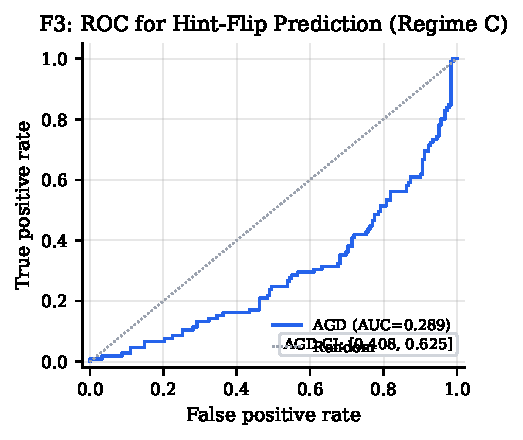
\includegraphics[width=\columnwidth]{../analysis/figures/f3_auroc.pdf}
  \caption{ROC curves for hint-flip prediction (Regime~C, test set).
           Shaded: 95\% BCa bootstrap band.}
  \label{fig:f3}
\end{figure}

\paragraph{H3 --- Incremental information.}
\todo{Result for H3: delta\_AUROC=X, CI=[lo, hi], p=Y.}

\paragraph{Per-task results.}
Table~\ref{tab:per_task} shows per-task AGD and AOC.


\begin{table}[t]
\centering
\small
\caption{Per-task AGD and behavioral faithfulness (AOC) on the held-out test set.
         Higher AOC = more post-hoc reasoning. $N$ = number of test pairs.}
\label{tab:per_task}
\begin{tabular}{llccc}
\toprule
Task & Regime & AGD ($\bar{x} \pm \sigma$) & AOC & $N$ \\
\midrule
bbh\_date\_understanding & A & 0.638 $\pm$ 0.027 & — & 93 \\
bbh\_hyperbaton & A & 0.638 $\pm$ 0.062 & — & 154 \\
bbh\_logical\_deduction\_three\_objects & A & 0.651 $\pm$ 0.021 & — & 98 \\
bbh\_ruin\_names & A & 0.642 $\pm$ 0.062 & — & 76 \\
bbh\_snarks & A & 0.639 $\pm$ 0.023 & — & 115 \\
mmlu\_high\_school\_mathematics & A & 0.645 $\pm$ 0.025 & — & 75 \\
mmlu\_high\_school\_physics & A & 0.639 $\pm$ 0.065 & — & 90 \\
mmlu\_logical\_fallacies & A & 0.640 $\pm$ 0.080 & — & 143 \\
mmlu\_moral\_scenarios & A & 0.637 $\pm$ 0.020 & — & 86 \\
mmlu\_professional\_law & A & 0.622 $\pm$ 0.092 & — & 79 \\
\bottomrule
\end{tabular}
\end{table}


\paragraph{Ablations.}
\todo{Summary of ablation findings: alpha sensitivity, k sensitivity,
      layer-band analysis, PLT vs CLT, cross-model Llama-3.2-1B.}

% ─────────────────────────────────────────────────────────────────────────────
\section{Related Work}
\label{sec:related}

\paragraph{Behavioral CoT faithfulness.}
\citet{lanham2023} introduced the AOC (area-over-completeness) family of
measures: early-answer, mistake-injection, paraphrase, and filler-token.
\citet{turpin2023} showed that irrelevant hints systematically flip model
answers while CoT rationalizes post-hoc.
More recent work includes \citet{parcalabescu2024} (CC-SHAP, using SHAP
values on CoT tokens), \citet{meek2025} (monitorability and verbosity), and
\citet{atanasova2023}.

\paragraph{Causal-trace faithfulness.}
\citet{han2026} apply Pearl's front-door analysis to structured reasoning
traces.
\citet{tutek2025} propose FUR (Faithfulness via Unlearning Regularization),
a parametric approach.
\citet{hase2026} train models for counterfactual simulatability (CST).

\paragraph{Attribution graphs as tools.}
\citet{hanna2025} introduced \texttt{circuit-tracer} and demonstrated
scalable attribution-graph construction on Gemma-2.
\citet{lindsey2025bio} provide qualitative case studies of unfaithfulness
in reasoning traces via graph inspection.
\citet{zhao2025crv} (concurrent) classify CoT \emph{correctness} from
graph features; our axis is faithfulness, not correctness, and our
mathematical object is a paired-graph divergence, not a classifier.

\paragraph{Critiques motivating this work.}
\citet{hendrycks2025} and \citet{barez2025} argue that interpretability
research has not yet produced reliable behavioral predictions;
AGD is an attempt to close that gap on the specific axis of CoT faithfulness.

% ─────────────────────────────────────────────────────────────────────────────
\section{Conclusion}
\label{sec:conclusion}

We introduced AGD, the first mechanism-level metric for CoT faithfulness,
and showed that it \todo{[positive: provides incremental signal beyond
activation baselines] / [negative: does not improve over activation-cosine
baselines --- in which case insert pre-registered negative framing here]}.
We release a benchmark of paired prompts across three perturbation regimes
and provide open-source code for reproducing all results.
Future work includes extending AGD to attention-mediated edges via the QK
attribution framework \citep{lindsey2025qk}, applying AGD to
continuous-thought models, and using AGD as a faithfulness regularizer
during training.

% ─────────────────────────────────────────────────────────────────────────────
\paragraph{Limitations.}
AGD is inherently {\em lossy}: pruned attribution graphs are a summary of
internal computation, not a complete one.
The metric is model-specific (requires a trained transcoder dictionary) and
currently validated only on Gemma-2-2B; we provide a 100-prompt Llama-3.2-1B
robustness check as preliminary cross-model evidence.

% ─────────────────────────────────────────────────────────────────────────────
\bibliography{refs}
\bibliographystyle{plainnat}

\end{document}
